%%%%%%%%%%%%%%%%%%%%%%%%%%%%%%%%%%%%%%%%%%%%%%%%%%%%%%%%%%
%   Autoren:
%   Prof. Dr. Bernhard Drabant
%   Prof. Dr. Dennis Pfisterer
%   Prof. Dr. Julian Reichwald
%%%%%%%%%%%%%%%%%%%%%%%%%%%%%%%%%%%%%%%%%%%%%%%%%%%%%%%%%%

%%%%%%%%%%%%%%%%%%%%%%%%%%%%%%%%%%%%%%%%%%%%%%%%%%%%%%%%%%
%	ANLEITUNG: 
%   1. Ersetzen Sie firmenlogo.jpg im Verzeichnis img
%   2. Passen Sie alle Stellen im Dokument an, die mit 
%      @stud 
%      markiert sind
%%%%%%%%%%%%%%%%%%%%%%%%%%%%%%%%%%%%%%%%%%%%%%%%%%%%%%%%%%

%%%%%%%%%%%%%%%%%%%%%%%%%%%%%%%%%%%%%%%%%%%%%%%%%%%%%%%%%%
%	ACHTUNG: 
%   Für das Erstellen des Literaturverzeichnisses wird das 
%   modernere Paket biblatex in Kombination mit biber 
%   verwendet - nicht mehr das ältere Paket BibTex!
%
%   Bitte stellen Sie Ihre TeX-Umgebung entsprechend ein (z.B. TeXStudio): 
%   Einstellungen --> Erzeugen --> Standard Bibliographieprogramm: biber
%%%%%%%%%%%%%%%%%%%%%%%%%%%%%%%%%%%%%%%%%%%%%%%%%%%%%%%%%%

\documentclass[fontsize=12pt,BCOR=5mm,DIV=12,parskip=half,listof=totoc,
               paper=a4,toc=bibliography,pointlessnumbers]{scrreprt}
               
\usepackage[utf8]{inputenc}

%% LANGUAGE SETTINGS
%
% @stud: Sprache ggf. anpassen
%
%\usepackage[ngerman]{babel} 	        % german language
%\usepackage[german=quotes]{csquotes} 	% correct quoting using \enquote{}
\usepackage[english]{babel}          % english language
\usepackage{csquotes} 	              % correct quoting using \enquote{}

%%%%%%%%%%%%%
%% ZITIERSTIL
%%%%%%%%%%%%%
%
% @stud: Zitierstil in package biblatex unten wählen
%
% NUMERIC Style - e. g. [12]
% style=numeric 
%
% IEEE Style - numeric kind of style 
% style=ieee 
%
% ALPHABETIC Style - e. g. [AB12]
% style=alphabetic 
%
% HARVARD Style 
% style=apa 
%
% CHICAGO Style 
% style=authoryear
%
% Position des Zitats:
%
% autocite=inline 
%
% (!!) FOOTNOTE POSITION NOT RECOMMENDED IN MINT DOMAIN:
% autocite=footnote
%
\usepackage[backend=biber, autocite=inline, style=numeric]{biblatex} 	
\usepackage{makeidx}                  % allows index generation
\usepackage{listings}	                %Format Listings properly
\usepackage{lipsum}                   % Blindtext
\usepackage{graphicx}                 % use various graphics formats
\usepackage[german]{varioref}         % nicer references \vref
\usepackage{caption}	                % better Captions
\usepackage{booktabs}                 % nicer Tabs
\usepackage[hidelinks=true]{hyperref} % keine roten Markierungen bei Links
\usepackage{fnpct}                    % Correct superscripts 
\usepackage{calc}                     % Used for extra space below footsepline, in particular
\usepackage{array}
\usepackage{acronym}
\usepackage{algorithm}
\usepackage{algpseudocode}
\usepackage{setspace}
\usepackage{tocloft}
\usepackage[T1]{fontenc}
\usepackage{tabularx}
\usepackage[utf8]{inputenc}

% Definitionen und Commands
\newcommand{\indextype}{numeric}
\newcommand{\abs}{\par\vskip 0.2cm\goodbreak\noindent}
\newcommand{\nl}{\par\noindent}
\newcommand{\mcl}[1]{\mathcal{#1}}
\newcommand{\nowrite}[1]{}
\newcommand{\NN}{{\mathbb N}}
\newcommand{\imagedir}{img}
\newcommand{\TitelDerArbeit}[1]{\def\DerTitelDerArbeit{#1}\hypersetup{pdftitle={#1}}}
\newcommand{\Dozent}[1]{\def\DerDozent{#1}}
\newcommand{\AutorDerArbeit}[1]{\def\DerAutorDerArbeit{#1}\hypersetup{pdfauthor={#1}}}
\newcommand{\Firma}[1]{\def\DerNameDerFirma{#1}}
\newcommand{\Kurs}[1]{\def\DieKursbezeichnung{#1}}
\newcommand{\Abteilung}[1]{\def\DerNameDerAbteilung{#1}}
\newcommand{\Studiengangsleiter}[1]{\def\DerStudiengangsleiter{#1}}
\newcommand{\WissBetreuer}[1]{\def\DerWissBetreuer{#1}}
\newcommand{\FirmenBetreuer}[1]{\def\DerFirmenBetreuer{#1}}
\newcommand{\Bearbeitungszeitraum}[1]{\def\DerBearbeitungszeitraum{#1}}
\newcommand{\Abgabedatum}[1]{\def\DasAbgabedatum{#1}}
\newcommand{\MatrikelnummerEins}[1]{\def\DieMatrikelnummerEins{#1}}
\newcommand{\MatrikelnummerZwei}[1]{\def\DieMatrikelnummerZwei{#1}}
\newcommand{\MatrikelnummerDrei}[1]{\def\DieMatrikelnummerDrei{#1}}
\newcommand{\Studienrichtung}[1]{\def\DieStudienrichtung{#1}}
\newcommand{\ArtDerArbeit}[1]{\def\DieArtDerArbeit{#1}}
\newcommand{\Literaturverzeichnis}{Literaturverzeichnis}

% Page Layout
\oddsidemargin=0mm
\evensidemargin=0mm
\textwidth=159mm
\topmargin=-18mm
\headsep=10mm
\textheight=251mm
\footheight=15mm

\makeindex

%%%%%%%%%%%%%%%%%%%%%%%%%%%%%%%%%%%
% LITERATURVERZEICHNIS
% @stud: Literaturverzeichnis in Datei bibliography.bib anpassen. 
%
% [Alternative zu Verwendung von \initializeBibliography: Citavi ... (dazu eigenes LaTex Coding verwenden)]
%
\addbibresource{bibliography.bib}
\DefineBibliographyStrings{ngerman}{andothers = {{et\,al\adddot}},}

% Elementare Konfigurationen und Definitionen werden geladen 
% @stud: gegebenenfalls anpassen
%
% !TEX root =  master.tex

%%%%%%%%%%%%%%%%%%%%%%%%%%%%%%%%%%%%%%%%%%%%%%%%%%%%%%%%%%%%%%%%%%
%	ANLEITUNG: 
% Passen Sie gegebenenfalls alle Stellen im Dokument an, die mit 
% @stud 
% markiert sind.
%%%%%%%%%%%%%%%%%%%%%%%%%%%%%%%%%%%%%%%%%%%%%%%%%%%%%%%%%%%%%%%%%%

%%
%% @stud
%%
%% LANGUAGE SETTINGS
\usepackage[english]{babel}          % english language
\usepackage{csquotes} 	              % correct quoting using \enquote{}
\usepackage{makeidx}                  % allows index generation
\usepackage{listings}	                % Format Listings properly
\usepackage{lipsum}                   % Blindtext
\usepackage{graphicx}                 % use various graphics formats
\usepackage[german]{varioref}         % nicer references \vref
\usepackage{caption}	                % better Captions
\usepackage{booktabs}                 % nicer Tabs
\usepackage[hidelinks=true]{hyperref} % keine roten Markierungen bei Links
\usepackage{fnpct}                    % Correct superscripts 
\usepackage{calc}                     % Used for extra space below footsepline, in particular
\usepackage{array}
\usepackage{acronym}
\usepackage{algorithm}
\usepackage{algpseudocode}
\usepackage{setspace}
\usepackage{tocloft}

%% Schriftarten- und Zeichenpakete
\usepackage[T1]{fontenc}
\usepackage[utf8]{inputenc}

%%
%% @stud
%%
%%	FONT SELECTION: Schriftarten und Schriftfamilie
%%%%%%%%%%%%%
%% SCHRIFTART
%%%%%%%%%%%%%
% 0) without decomment: normal font families 
% ...
% 1) Latin Modern 
%\usepackage{lmodern}        
% 2) Times 
%\usepackage{mathptmx}         
% 3) Helvetica
%\usepackage[scaled=.92]{helvet} 
%%%%%%%%%%%%%%%%%%
%%	SCHRIFTFAMILIE
%%%%%%%%%%%%%%%%%%
% ohne Serifen
\renewcommand*{\familydefault}{\sfdefault}
\addtokomafont{disposition}{\sffamily}
%
% mit Serifen
%\renewcommand*{\familydefault}{\rmdefault}
%\addtokomafont{disposition}{\rmfamily}
%
% Typewriter
%\renewcommand*{\familydefault}{\ttdefault}
%\addtokomafont{disposition}{\ttfamily}

%%
%% @stud
%%
%% Uncomment the following lines to support hard URL breaks in bibliography 
%\apptocmd{\UrlBreaks}{\do\f\do\m}{}{}
%\setcounter{biburllcpenalty}{9000}% Kleinbuchstaben
%\setcounter{biburlucpenalty}{9000}% Großbuchstaben

%%
%% @stud
%%
%% FOOTNOTES: Count footnotes over chapters
%% \counterwithout{footnote}{chapter}

%	ACRONYMS
\makeatletter
\@ifpackagelater{acronym}{2015/03/20}
{\renewcommand*{\aclabelfont}[1]{\textbf{{\acsfont{#1}}}}}{}
\makeatother

%	LISTINGS
% @stud: ggf. Namen/Text anpassen (englisch)
\renewcommand{\lstlistingname}{Quelltext} 
\renewcommand{\lstlistlistingname}{Quelltextverzeichnis}
\lstset{numbers=left,
	numberstyle=\tiny,
	captionpos=b,
	basicstyle=\ttfamily\small}

%	ALGORITHMS
% @stud: ggf. Namen/Text anpassen (englisch)
\renewcommand{\listalgorithmname}{Algorithmenverzeichnis}
\floatname{algorithm}{Algorithmus}

%	PAGE HEADER / FOOTER
%	Warning: There are some redefinitions throughout the master.tex-file!  DON'T CHANGE THESE REDEFINITIONS!
\RequirePackage[automark]{scrlayer-scrpage}
%alternatively with separation lines: \RequirePackage[automark,headsepline,footsepline]{scrlayer-scrpage}

\renewcommand{\chaptermarkformat}{}
\RedeclareSectionCommand[beforeskip=0pt]{chapter}
\clearpairofpagestyles

%\ifoot[\rule{0pt}{\ht\strutbox+\dp\strutbox}DHBW Mannheim]{\rule{0pt}{\ht\strutbox+\dp\strutbox}DHBW Mannheim}
\ofoot[\rule{0pt}{\ht\strutbox+\dp\strutbox}\pagemark]{\rule{0pt}{\ht\strutbox+\dp\strutbox}\pagemark}
\ohead{\headmark}

%\newcommand{\TitelDerArbeit}[1]{\def\DerTitelDerArbeit{#1}\hypersetup{pdftitle={#1}}}
%\newcommand{\AutorDerArbeit}[1]{\def\DerAutorDerArbeit{#1}\hypersetup{pdfauthor={#1}}}
%\newcommand{\Firma}[1]{\def\DerNameDerFirma{#1}}
%\newcommand{\Kurs}[1]{\def\DieKursbezeichnung{#1}}
%\newcommand{\Abteilung}[1]{\def\DerNameDerAbteilung{#1}}
%\newcommand{\Studiengangsleiter}[1]{\def\DerStudiengangsleiter{#1}}
%\newcommand{\WissBetreuer}[1]{\def\DerWissBetreuer{#1}}
%\newcommand{\FirmenBetreuer}[1]{\def\DerFirmenBetreuer{#1}}
%\newcommand{\Bearbeitungszeitraum}[1]{\def\DerBearbeitungszeitraum{#1}}
%\newcommand{\Abgabedatum}[1]{\def\DasAbgabedatum{#1}}
%\newcommand{\Matrikelnummer}[1]{\def\DieMatrikelnummer{#1}}
%\newcommand{\Studienrichtung}[1]{\def\DieStudienrichtung{#1}}
%\newcommand{\ArtDerArbeit}[1]{\def\DieArtDerArbeit{#1}}
%\newcommand{\Literaturverzeichnis}{Literaturverzeichnis}

\newcommand{\settingBibFootnoteCite}{
	\setlength{\bibparsep}{\parskip}		  % Add some space between biblatex entries in the bibliography
	\addbibresource{bibliography.bib}	    % Add file bibliography.bib as biblatex resource
	\DefineBibliographyStrings{ngerman}{andothers = {{et\,al\adddot}},}
}

\newcommand{\setTitlepage}{
	% !TEX root =  master.tex
% @stud: ggf. Namen/Text anpassen (englisch)
\begin{titlepage}
\begin{minipage}{\textwidth}
		\vspace{-2cm}
		\noindent \hfill 
\includegraphics{\imagedir/logo.jpg}
\end{minipage}
\vspace{1em}
%\sffamily
\begin{center}
	{\textsf{\large Duale Hochschule Baden-W\"urttemberg Mannheim}}\\[4em]
	{\textsf{\textbf{\large{\DieArtDerArbeit}arbeit}}}\\[6mm]
	{\textsf{\textbf{\Large{}\DerTitelDerArbeit}}} \\[1.5cm]
	{\textsf{\textbf{\large{}Studiengang Informatik}}\\[6mm]
	\textsf{\textbf{Studienrichtung \DieStudienrichtung}}}\vspace{10em}
	
	\begin{minipage}{\textwidth}
		\begin{tabbing} 
		Wissenschaftliche(r) Betreuer(in): \hspace{0.85cm}\=\kill
		Verfasser(in): \> \DerAutorDerArbeit \\[1.5mm] 
		Matrikelnummer: \> \DieMatrikelnummerEins \\[1.5mm]
		Matrikelnummer: \> \DieMatrikelnummerZwei \\[1.5mm]
		Matrikelnummer: \> \DieMatrikelnummerDrei \\[1.5mm]
		%Firma: \> \DerNameDerFirma  \\[1.5mm]
		%Abteilung: \> \DerNameDerAbteilung \\[1.5mm]
		Kurs: \> \DieKursbezeichnung \\[1.5mm]
		Dozent: \> \DerDozent\\[1.5mm]
		%Studiengangsleiter: \> \DerStudiengangsleiter \\[1.5mm]
		%Wissenschaftliche(r) Betreuer(in): \> \DerWissBetreuer \\[1.5mm]
		%Firmenbetreuer(in): \> \DerFirmenBetreuer \\[1.5mm]
		Bearbeitungszeitraum: \> \DerBearbeitungszeitraum\\[1.5mm]
		
%		alternativ:\\[1.5mm]
%		Eingereicht: \> \DasAbgabedatum	
		\end{tabbing}
	\end{minipage}
\end{center}
\end{titlepage}
	\pagenumbering{roman} % Römische Seitennummerierung
	\normalfont	
}

\newcommand{\initializeText}{
	\clearpage
	\ihead{\chaptername~\thechapter} % Neue Header-Definition
	\pagenumbering{arabic}           % Arabische Seitenzahlen
}

\newcommand{\initializeBibliography}{
	\ihead{}
	\printbibliography[title=\Literaturverzeichnis] 
	\cleardoublepage
}

\newcommand{\initializeAppendix}{
	\appendix
  \ihead{}
  \cftaddtitleline{toc}{chapter}{Anhang}{}
}



% @stud
%
% PERSÖNLICHE ANGABEN (BITTE VOLLSTÄNDIG EINGEBEN zwischen den Klammern: {...})
%
\ArtDerArbeit{Projektbericht} % "Bachelor" oder "Projekt" wählen
\TitelDerArbeit{Intel Core I7 Prozessoren}
\AutorDerArbeit{Moritz Werr, Phil Richter, Max Stege}
\Abteilung{<Ihre Abteilung>}
\Firma{<Ihre Firma>}
\Kurs{TINF22AI2}
\Studienrichtung{Angewandte Informatik}
\MatrikelnummerEins{5401527}
\MatrikelnummerZwei{4164342}
\MatrikelnummerDrei{7285772}
\Studiengangsleiter{<Ihr Studiengangsleiter>}
\WissBetreuer{<Ihr(e) wissenschaftliche(r) Betreuer(in)>}
\FirmenBetreuer{<Ihr(e) Firmenbetreuer(in)>}
\Dozent{Dr. Frank Schulz}
\Bearbeitungszeitraum{01.10.2024 -- 01.12.2024}
\Abgabedatum{dd.mm.yyyy}

\begin{document}

\setTitlepage

%%%%%%%%%%%%%%%%%%%%%%%%%%%%%%%%%%%
% EHRENWÖRTLICHE ERKLÄRUNG
%
% @stud: ewerkl.tex bearbeiten
%
% !TEX root =  master.tex
\clearpage
\chapter*{Ehrenwörtliche Erklärung}

% Wird die folgende Zeile auskommentiert, erscheint die ehrenwörtliche
% Erklärung im Inhaltsverzeichnis.

% \addcontentsline{toc}{chapter}{Ehrenwörtliche Erklärung}
Ich versichere hiermit, dass ich die vorliegende Arbeit mit dem Titel ``\textit{\DerTitelDerArbeit}'' selbstständig verfasst und 
keine anderen als die angegebenen Quellen und Hilfsmittel benutzt habe. Ich versichere zudem, dass die eingereichte elektronische 
Fassung mit der gedruckten Fassung übereinstimmt.

\vspace{3cm}
%Ort, Datum \hfill \DerAutorDerArbeit
 
\cleardoublepage  
%%%%%%%%%%%%%%%%%%%%%%%%%%%%%%%%%%%

%%%%%%%%%%%%%%%%%%%%%%%%%%%%%%%%%%%
% SPERRVERMERK
%
% @stud: nondisclosurenotice.tex bearbeiten
%
%%%%%%%%%%%%%%%%%%%%%%%%%%%%%%%%%%%

%%%%%%%%%%%%%%%%%%%%%%%%%%%%%%%%%%%
%	KURZFASSUNG
%
% @stud: acknowledge.tex bearbeiten
%
%%%%%%%%%%%%%%%%%%%%%%%%%%%%%%%%%%%

%%%%%%%%%%%%%%%%%%%%%%%%%%%%%%%%%%%
% VERZEICHNISSE und ABSTRACT
%
% @stud: ggf. nicht benötigte Verzeichnisse auskommentieren/löschen
%
%	Listingsverzeichnis / Quelltextverzeichnis
\lstlistoflistings
\cleardoublepage
\onehalfspacing
\initializeText

%%%%%%%%%%%%%%%%%%%%%%%%%%%%%%%%%%%%%%%%%%%%%%%%%%%%%%%%%%%%%%%%%%%%%%%%%%%%%%%%%%%%%%%%%%
% KAPITEL UND ANHÄNGE
%
% @stud:
%   - nicht benötigte: auskommentieren/löschen
%   - neue: bei Bedarf hinzufügen mittels input-Kommando an entsprechender Stelle einfügen
%%%%%%%%%%%%%%%%%%%%%%%%%%%%%%%%%%%%%%%%%%%%%%%%%%%%%%%%%%%%%%%%%%%%%%%%%%%%%%%%%%%%%%%%%%

%%%%%%%%%%%%%%%%%%%%%%%%%%%%%%%%%%%
% KAPITEL
%
% @stud: einzelne Kapitel bearbeiten und eigene Kapitel hier einfügen
%
% Einleitung
% !TEX root =  master.tex
\chapter{Einleitung (Max Stege)}

\nocite{*}

Die rasante Entwicklung der Computertechnologie wird seit Jahrzehnten von einer zentralen Beobachtung geprägt: dem Mooreschen Gesetz. Dieses Gesetz postuliert, dass sich die Anzahl der Transistoren auf integrierten Schaltkreisen etwa alle zwei Jahre verdoppelt, was zu exponentiellen Leistungssteigerungen bei gleichzeitiger Reduzierung der Kosten führt \cite{noauthor_moores_nodate}. Doch angesichts physikalischer und technischer Grenzen wird zunehmend diskutiert, ob dieses Gesetz auch heute noch seine Gültigkeit hat. Die Analyse der Entwicklung von Prozessoren, wie der Intel Core i7-Reihe, bietet eine spannende Möglichkeit, diese Frage aus einer datengetriebenen Perspektive zu untersuchen.

Neben der Überprüfung des Mooreschen Gesetzes steht die Frage im Fokus, in welchen Bereichen die größten Fortschritte erzielt wurden. Hat die Erhöhung der Kernanzahl maßgeblich zur Leistungssteigerung beigetragen, oder sind es optimierte Taktraten und eine verbesserte Energieeffizienz, die den Unterschied ausmachen? Gleichzeitig wird analysiert, welche Metriken über die Generationen hinweg stagniert sind und welche Faktoren möglicherweise als limitierende Größen der technologischen Entwicklung wirken.

Dieses Projekt, durchgeführt im Rahmen der Vorlesung \textit{Big Data Analytics}, widmet sich der strukturierten Analyse und Visualisierung von Daten zu Intel Core i7-Prozessoren der letzten Generationen. Dabei soll nicht nur der technische Fortschritt dokumentiert werden, sondern auch ein umfassendes Verständnis für die Datengrundlage und deren Interpretation entwickelt werden. Um dies zu ermöglichen, wurde eine mehrstufige Pipeline realisiert, die sich über folgende Schritte erstreckt:

\begin{itemize}
    \item \textbf{Datenbeschaffung:} Sammlung technischer Spezifikationen direkt von der Herstellerwebsite, da keine öffentliche API verfügbar ist.
    \item \textbf{Datenaufbereitung:} Transponierung und Bereinigung der Rohdaten, um diese für die weitere Analyse nutzbar zu machen.
    \item \textbf{Datenbankintegration:} Speicherung der Daten in einer relationalen PostgreSQL-Datenbank, um eine flexible und effiziente Abfrage der Datensätze zu ermöglichen.
    \item \textbf{Analyse und Visualisierung:} Nutzung moderner Datenanalyse- und Visualisierungs- werkzeuge, um Muster und Trends über verschiedene Prozessorgenerationen hinweg zu identifizieren.
\end{itemize}

Durch diese strukturierte Herangehensweise können entscheidende Fragen beantwortet werden: Welche Metriken zeigen die stärksten Fortschritte? Wo sind technologische Grenzen erreicht? Und welche Entwicklungen könnten in den kommenden Jahren dominieren? Die gewonnenen Erkenntnisse liefern nicht nur einen detaillierten Überblick über die Entwicklung der Intel Core i7-Serie, sondern geben auch Impulse für zukünftige Innovationen und die strategische Ausrichtung der Halbleiterindustrie.

Diese Dokumentation beschreibt im Detail den technischen und methodischen Ablauf des Projekts. Ziel ist es, eine nachvollziehbare und robuste Datenpipeline zu präsentieren, die als Grundlage für weiterführende Analysen und Forschungsprojekte dienen kann. Darüber hinaus wird kritisch reflektiert, welche Limitierungen und Herausforderungen sich in der Umsetzung ergeben haben, und wie diese überwunden werden können.


% mehrere Grundlagen- und Forschungs-Kapitel
% !TEX root =  master.tex
\chapter{Vorbereitung der Daten}

Intel bietet auf ihrer Webseite die Möglichkeit unterschiedliche Prozessoren miteinander zu vergleichen.
Es werden alle Desktop-Prozessoren der Intel Core I7-Reihe an Prozessoren ausgewählt, damit es eine große Anzahl an Datensätzen gibt und auch die Spannweite zwischen gewissen Werten groß genug ist, dass Unterschiede leichter zu erkennen sind.
Z.B. ist die Kernanzahl pro Prozessor seit der 4. Generation stark gestiegen, wohingegen die Anzahl an Prozessorkernen bei Intel Core I3-Modellen nicht so stark angestiegen sind.
Die Daten werden direkt von \href{https://www.intel.de/content/www/de/de/products/compare.html?productIds=212279,212280,212047,212048,212251,199325,199335,199314,199316,199318,191048,191792,193738,190885,186604,148263,140642,126684,97129,93339,88200,88195,87718,88040,80807,80808,80809,80814,80806,77656,76642,75121,75122,75123,75124,75125,236781,236794,236854,236783,236789,230492,230490,230491,230500,230489,134596,134591,134592,134594,134595,129948,126686,97122,97128,88196}{Intels Webseite} bezogen.
Da Intel keine öffentliche API anbietet, um deren CPU-Spezifikationen zu vergleichen und zu exportieren, muss die CSV-Datei selber heruntergeladen werden. 
Bevor die Daten aus der CSV ausgelesen werden können, müssen diese noch etwas aufbereitet werden.
Wie in Abbildung \ref{fig:intel_webseite} von der Herstellerseite zu sehen ist, sind hier leider die Prozessormodelle die Spalten anstatt der Zeilen. 


Bevor die CSV bereinigen können, muss also die  Matrix der CSV noch einmal transponiert werden.
Sonst wären die einzelnen Prozessoren die Spalten in der Datenbank, in der die bereinigte Daten der CSV abgespeichert werden.
Weiterhin sind nicht alle Spalten in der CSV interessant für die Auswertung der Daten.
Viele der Einträge in der CSV listen nur Features oder Prozessorerweiterungen auf, die nicht einfach zu vergleichen sind oder sich nur schwierig visualisieren lassen.
Weiterhin sind manche Einträge bei älteren Prozessoren komplett leer, weswegen die Datenmenge in diesen Spalten sehr gering ist.
Daher werden nur ausgewählte Spalten gespeichert, die für die Fragestellung interessant sind und auch genügend Datenpunkte haben.

\cleardoublepage

\begin{figure}
	\centering 
	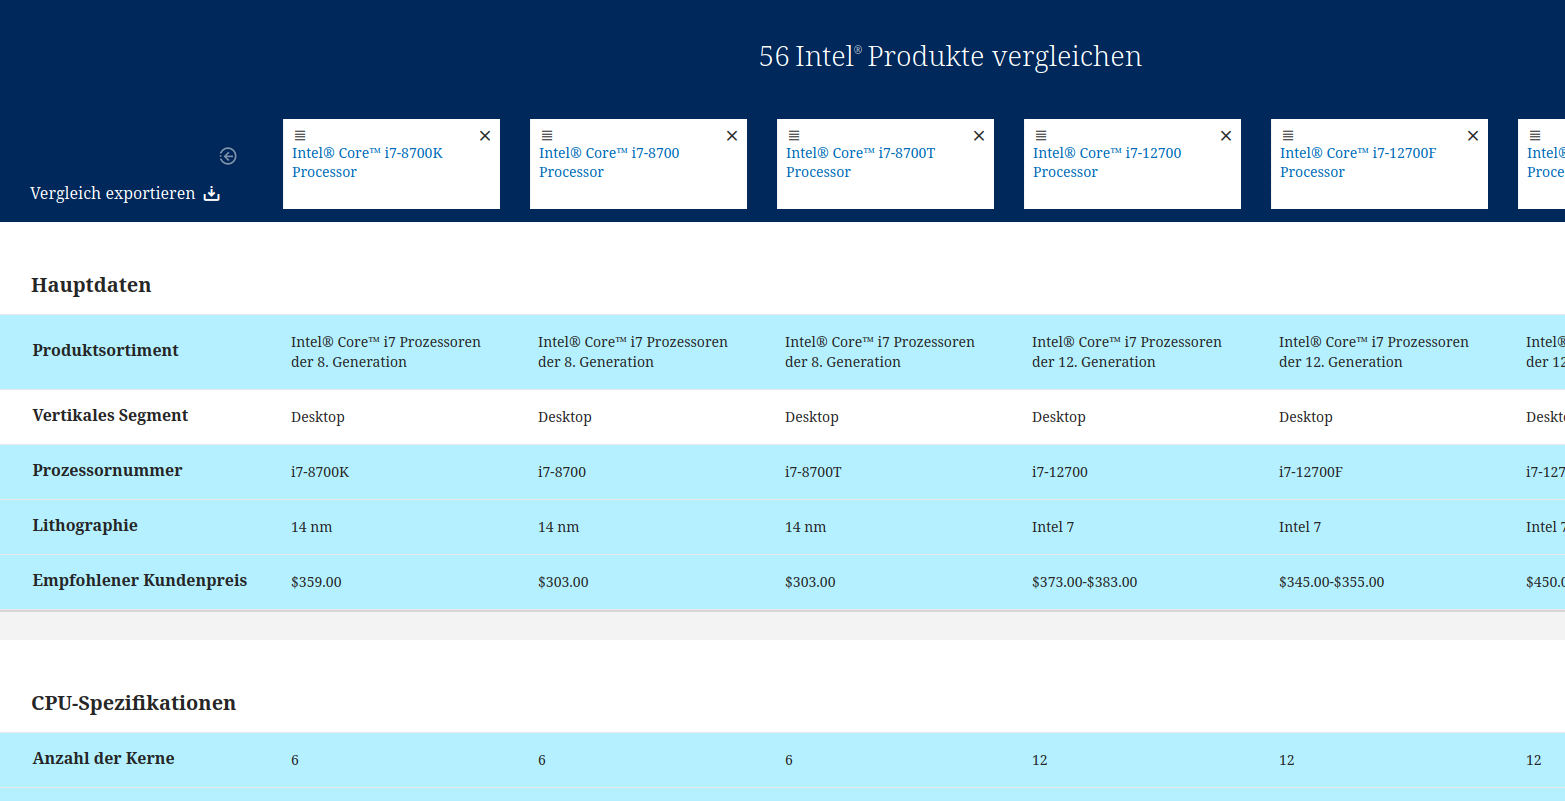
\includegraphics[width=\textwidth]{\imagedir/webseite.png} 
	\captionsetup{format=hang}
	\caption[Webseite von Intel]{\label{fig:intel_webseite}Webseite zum Produktvergleich von Intel-Prozessoren \\Quelle: \cite{i7_intel_2024}}
\end{figure}

Aufgrund der mächtigen Standardwerkzeugen eines POSIX-kompatiblen Betriebssystem wie Linux, wurde \lstinline |awk| verwendet, um die Spalten in Zeilen zu konvertieren bzw. die Zeilen zu Spalten zu konvertieren.
\lstinline |awk| ist ein Werkzeug zur Erkennung und Verarbeitung von Textmustern \cite{noauthor_awk1_nodate}.
\lstinline |awk| arbeitet nicht nur mit Zeilen, wie z.B. \lstinline |grep| oder \lstinline |sed|, sondern kann auch in einzelnen Spalten bzw. Feldern filtern \cite{noauthor_awk1_nodate}.
Normalerweise sind die Standardtrennzeichen von Spalten für \lstinline |awk|  Leerzeichen und Tabulatoren. Es ist aber möglich mit dem `-F` Flag anzugeben, dass ein anderes Trennzeichen verwendet wird \cite{noauthor_awk1_nodate}.
In unserem Fall wird das Trennzeichen das Komma sein, weil wir mit einer CSV arbeiten.
In \lstinline |awk| wird häufig mit regulären Ausdrucken gefiltert, aber da unsere Datei eine statische CSV-Datei ist, kann direkt nach Spaltennamen sortiert werden.
Das entsprechende Skript sieht folgendermaßen aus:

\begin{lstlisting}[caption={\texttt{clean.sh}},captionpos=b]
#!/bin/bash

awk -F ',' '
NR==5   ||
NR==7   ||
NR==8   ||
NR==12  ||
NR==13  ||
NR==14  ||
NR==15  ||
NR==16  ||
NR==17  ||
NR==18  ||
NR==19  ||
NR==22  ||
NR==23  ||
NR==24  ||
NR==25  ||
NR==26  ||
NR==27  ||
NR==28  ||
NR==29  ||
NR==30  ||
NR==31  ||
NR==36  ||
NR==42  ||
NR==56  ||
NR==57  ||
NR==58  ||
NR==59  ||
NR==60  ||
NR==61  ||
NR==62  ||
NR==82  ||
NR==90 
{print $0}' "Intel_UPE_ComparisonChart_2024_11_04_i7.csv" |

awk '
{
	for (i=1; i<=NF; i++)  
	a[i] = a[i] ? a[i] "," $i : $i  
}
END {
	for (i=1; i in a; i++)  
	print a[i]
}
' FS=, OFS=, > clean.csv
\end{lstlisting}

Das Skript besteht aus zwei Teilen: Im ersten Teil werden die entsprechenden Spalten mit \lstinline |awk| nach Spaltennummer ausgefiltert, welche vorher als interessant deklariert wurden, und in den zweiten Teil gepiped. 
Im zweiten Teil werden die jeweiligen Spalten in einer for-Schleife in neue Zeilen geladen. Nachdem die gesamte Datei eingelesen wurde, kann diese wieder transponiert ausgegeben werden. Nun kann mit dem eigentlichen Säubern der Daten begonnen werden.




% !TEX root =  master.tex
\chapter{Säubern der Daten}

Nun ist die CSV vorbereitet für die eigentliche Säuberung. Die Daten liegen in den entsprechenden Spalten vor und alle uninteressanten Daten wurden entfernt.
Bevor die Daten jedoch in einer Datenbank in Tabellenform gespeichert werden können, sollten noch entsprechende Spalten bereinigt werden, dass nur noch Zahlenwerte ohne Einheiten dort aufzufinden sind.
Weiterhin beinhalten viele Spaltennamen immer noch Sonderzeichen und Leerzeichen, welche es schwierig macht die Spalten zu lesen.

Um diese Probleme zu addressieren, wurde R zur Bereinigung der Daten ausgewählt.
R ist eine Skriptsprache für statistische Berechnungen \cite{noauthor_r_nodate}. Es bietet mächtige Werkzeuge zur Auswertung und Speicherung von Daten \cite{noauthor_r_nodate}. Damit ist damit eine exzellente Wahl um dieses Problem zu lösen.
Es bietet Möglichkeiten die Spaltennamen automatisch mit der Funktion  \lstinline |clean_names()| aus der Bibliothek \lstinline|janitor| umzubenennen \cite{noauthor_janitor_nodate}, indem es problematische Zeichen, wie z.B. Leerzeichen und Sonderzeichen, erkennt und durch unproblematische Zeichen ersetzt.
Weiterhin werden auch alle Großbuchstaben durch Kleinbuchstaben ersetzt.
Darüber hinaus ist R eine dynamisch typisierte Skriptsprache. Datentypen werden je nach Kontext automatisiert erkannt.
Wenn die entsprechenden Spalten von allen nicht-numerischen Zeichen gesäubert werden, lassen sich diese problemlos in Zahlen umwandeln.
Die entsprechenden Einheiten werden nach der Spaltensäuberung stattdessen noch in den Spaltennamen hinzugefügt.

Wenn alle Spalten und Spaltennamen gesäubert bzw. angepasst wurden, können die Daten in einer Datenbank gespeichert werden.

Mit den vorher genannten Überlegungen im Hinterkopf ist folgendes Skript entstanden: 


\lstset{
	breaklines=true,         % Enable line wrapping
	breakatwhitespace=false, % Allow breaks at any character (not just whitespace)
	basicstyle=\ttfamily,    % Use monospaced font
}

\begin{lstlisting}[caption={\texttt{database.R}},captionpos=b]
#!/usr/bin/Rscript

library(RPostgres)

intel <- read.csv("clean.csv")		#Reading
intel <- janitor::clean_names(intel)	#Cleaning the column names

#cleaning and mutating columns to numbers
intel$max_turbo_taktfrequenz <- as.numeric(gsub(" GHz", "", intel$max_turbo_taktfrequenz))
intel$lithographie <- gsub("Intel 7", "10 nm", intel$lithographie)
intel$lithographie <- as.numeric(gsub(" nm", "", intel$lithographie))
intel$intel_turbo_boost_technik_2_0_taktfrequenz <- as.numeric(gsub(" GHz", "", intel$intel_turbo_boost_technik_2_0_taktfrequenz))
intel$grundtaktfrequenz_des_prozessors <- gsub(" \\| ", ".", intel$grundtaktfrequenz_des_prozessors)
intel$grundtaktfrequenz_des_prozessors <- as.numeric(gsub(" GHz", "", intel$grundtaktfrequenz_des_prozessors))
intel$cache <- gsub(" MB Intel Smart Cache", "", intel$cache)
intel$cache <- as.numeric(gsub(" MB", "", intel$cache))
intel$bus_taktfrequenz <- as.numeric(gsub(" GT/s", "", intel$bus_taktfrequenz))
intel$verlustleistung_tdp <- as.numeric(gsub(" W", "", intel$verlustleistung_tdp))
intel$intel_turbo_boost_max_technology_3_0_frequency <- gsub(" \\| ", ".", intel$intel_turbo_boost_max_technology_3_0_frequency)
intel$intel_turbo_boost_max_technology_3_0_frequency <- as.numeric(gsub(" GHz", "", intel$intel_turbo_boost_max_technology_3_0_frequency))
intel$single_p_core_turbo_frequency <- as.numeric(gsub(" GHz", "", intel$single_p_core_turbo_frequency))
intel$single_e_core_turbo_frequency <- as.numeric(gsub(" GHz", "", intel$single_e_core_turbo_frequency))
intel$e_core_base_frequency <- gsub(" GHz", "", intel$e_core_base_frequency)
intel$e_core_base_frequency <- as.numeric(gsub("900 MHz", "0.9", intel$e_core_base_frequency))
intel$total_l2_cache <- as.numeric(gsub(" MB", "", intel$total_l2_cache))
intel$processor_base_power <- as.numeric(gsub(" W", "", intel$processor_base_power))
intel$maximum_turbo_power <- as.numeric(gsub(" W", "", intel$maximum_turbo_power))
intel$grundtaktfrequenz_der_grafik <- as.numeric(gsub(" MHz", "", intel$grundtaktfrequenz_der_grafik))
intel$max_dynamische_grafikfrequenz <- as.numeric(gsub(" GHz", "", intel$max_dynamische_grafikfrequenz))
intel$max_videospeicher_der_grafik <- as.numeric(gsub(" GB", "", intel$max_videospeicher_der_grafik))
intel$x4k_unterstutzung <- gsub("Hz", "", intel$x4k_unterstutzung)
intel$x4k_unterstutzung <- as.numeric(gsub("Yes \\|  at ", "", intel$x4k_unterstutzung))


#Putting the units back into the column names
colnames(intel)[colnames(intel) == "max_turbo_taktfrequenz"] <- "max_turbo_taktfrequenz_GHz"
colnames(intel)[colnames(intel) == "lithographie"] <- "litographie_nm"
colnames(intel)[colnames(intel) == "intel_turbo_boost_technik_2_0_taktfrequenz"] <- "intel_turbo_boost_technik_2_0_taktfrequenz_GHz"
colnames(intel)[colnames(intel) == "grundtaktfrequenz_des_prozessors"] <- "grundtaktfrequenz_des_prozessors_GHz"
colnames(intel)[colnames(intel) == "cache"] <- "cache_MB"
colnames(intel)[colnames(intel) == "bus_taktfrequenz"] <- "bus_taktfrequenz_GT_per_s"
colnames(intel)[colnames(intel) == "verlustleistung_tdp"] <- "verlustleistung_tdp_W"
colnames(intel)[colnames(intel) == "intel_turbo_boost_max_technology_3_0_frequency"] <- "intel_turbo_boost_max_technology_3_0_frequency_GHz"
colnames(intel)[colnames(intel) == "single_p_core_turbo_frequency"] <- "single_p_core_turbo_frequency_GHz"
colnames(intel)[colnames(intel) == "single_e_core_turbo_frequency"] <- "single_e_core_turbo_frequency_GHz"
colnames(intel)[colnames(intel) == "e_core_base_frequency"] <- "e_core_base_frequency_GHz"
colnames(intel)[colnames(intel) == "total_l2_cache"] <- "total_l2_cache_MB"
colnames(intel)[colnames(intel) == "processor_base_power"] <- "processor_base_power_W"
colnames(intel)[colnames(intel) == "maximum_turbo_power"] <- "maximum_turbo_power_W"
colnames(intel)[colnames(intel) == "grundtaktfrequenz_der_grafik"] <- "grundtaktfrequenz_der_grafik_MHz"
colnames(intel)[colnames(intel) == "max_dynamische_grafikfrequenz"] <- "max_dynamische_grafikfrequenz_GHz"
colnames(intel)[colnames(intel) == "max_videospeicher_der_grafik"] <- "max_videospeicher_der_grafik_GB"
colnames(intel)[colnames(intel) == "x4k_unterstutzung"] <- "x4k_unterstutzung_at"


con <- dbConnect(
RPostgres::Postgres(),
dbname = "bda",
host = "localhost" ,
port = 5432,
user = "bda",
password = "bda",
)

dbWriteTable(con, "intel", intel, row.names = FALSE, overwrite = TRUE)
dbDisconnect(con)
\end{lstlisting}

Als erstes wird die transponierte CSV eingelesen und die Spaltennamen mit Hilfe der `janitor` Library gesäubert. Danach kommt ein großer Block an Funktionen, die die einzelnen Spalten von Einheiten und komischer Formatierung säubern.
Danach kommt ein großer Block zur Umbenennung der Spaltennamen. 
Im letzten Schritt wird der Dataframe in einer existierenden Datenbank gespeichert. 
Ein großer Vorteil an der Funktion ist, dass die Tabelle innerhalb der Datenbank vorher nicht existieren muss. 
R erstellt von selber eine neue Tabelle mit entsprechenden Datentypen basierend auf den Datentypen innerhalb des Dataframes. Daher ist es wichtig die Daten innerhalb des Skripts schon zu Nummern zu konvertieren.

% !TEX root =  master.tex
\chapter{Speichern der Daten (Moritz Werr)}

Aus dem vorherigen Kapitel ist bereits hervorgegangen, dass die Daten in einer Datenbank gespeichert werden.
In diesem Fall ist die Wahl auf PostgreSQL gefallen.
PostgreSQL ist ein Open-Source, relationales Datenbankmanagementsystem \cite{noauthor_postgresql_nodate}. Es ist komplett ACID-kompatibel \cite{noauthor_postgresql_nodate} und speichert Daten in geordneter Form als Tabellen ab \cite{noauthor_51_2024}.
Da die Datenquelle bereits als CSV geliefert wird, bietet es sich an diese in einer entsprechenden Datenbank zu speichern.
CSV-Dateien speichern bereits Daten in Tabellenform, weswegen die Wahl direkt auf eine relationale SQL-Datenbank gefallen ist.

Es gibt viele Alternativen zu PostgreSQL, diese sind aber teils kostenpflichtig oder bieten die gleichen bzw. weniger Features wie PostgreSQL.
Proprietäre Datenbankmanagementsysteme wie Oracle RDBMS oder Microsoft SQL-Server sind für große, Enterprise-Skala Deployments konzipiert und entsprechend kommerzielle Lizenzen \cite{noauthor_microsoft_nodate}\cite{noauthor_oracle_nodate}.
Kostenlose Optionen sind daher bevorzugt.
MariaDB bzw. MySQL und SQLite wären Open-Source Alternativen zu PostgreSQL, welche auch gut geeignet sind\cite{noauthor_sqlite_nodate}\cite{noauthor_mysql_nodate}.
SQLite jedoch bietet keine Serverfunktionalität weswegen nur lokal gearbeitet werden kann\cite{noauthor_sqlite_nodate}.
MariaDB/MySQL haben keinen nennenswerten Funktionalitätsunterschied, aber wurden nicht gewählt, weil mit PostgreSQL mehr Erfahrung im Team existiert\cite{noauthor_mysql_nodate}\cite{noauthor_postgresql_nodate-1}.

Nachdem das Skript aus dem vorherigen Kapitel durchgelaufen ist, ist das Datenbankschema in Abbildung \ref{fig:datenbankschema} zu sehen.

\begin{figure}
	\centering 
	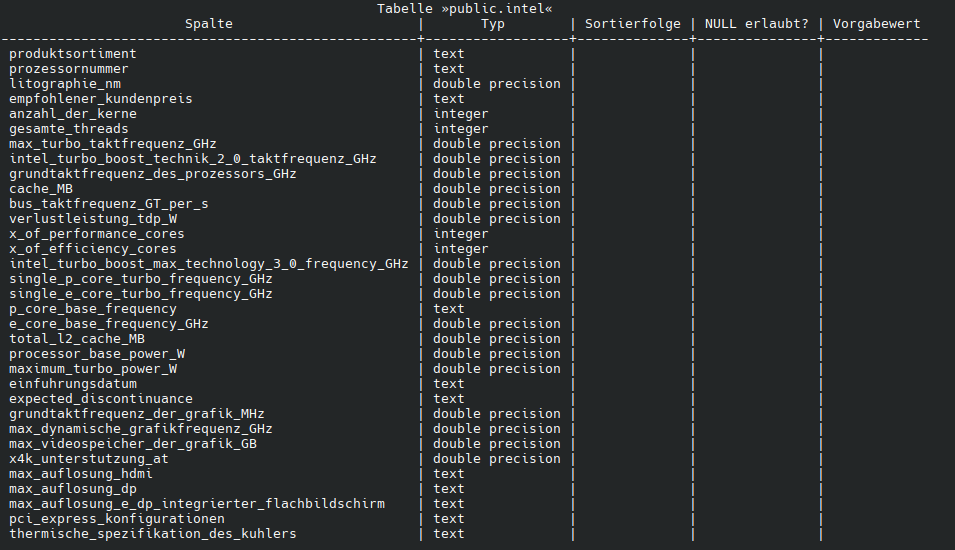
\includegraphics[width=\textwidth]{\imagedir/datenbank_schema.png} 
	\captionsetup{format=hang}
	\caption[Datenbankschema]{\label{fig:datenbankschema}Datenbankschema erstellt durch das R-Skript}
\end{figure}
% !TEX root =  master.tex
\chapter{Visualisieren der Daten (Phil Richter)}
Nach der Bereinigung und dem Speichern der Daten in einer Datenbank, wie in den vorherigen Kapiteln beschrieben, können die Daten visualisiert werden. Dafür wird als Grundlage
die Programmiersprache Python mit der Version 3.12.7 verwendet \cite{noauthor_python_nodate}. Diese ist vorallem im Bereich der Datenanalyse und -visualisierung sehr weit
verbreitet \cite{noauthor_most_nodate, noauthor_popular_nodate}. Eine alternative Möglichkeit wäre die Verwendung von R, welches ebenfalls sehr weit verbreitet ist und speziell
für die Datenanalyse entwickelt wurde \cite{noauthor_r_nodate}. Zudem wurde R bereits für die Säuberung der Daten, wie im Kapitel \ref{chap:säubern} beschrieben, verwendet.
Da im Team allerdings mehr Erfahrung mit Python vorhanden war, wurde sich bei der Visualsierung für die Verwendung von Python entschieden.

Für das Laden und Visualisiern der Daten werden folgende Packages verwendet:
\begin{table}[h!]
    \centering
    \begin{tabularx}{\textwidth}{|c|c|>{\centering\arraybackslash}X|}
        \hline
        \textbf{Package} & \textbf{Version} & \textbf{Beschreibung} \\ \hline
        dotenv & 1.0.1 & Lädt Umgebungsvariablen aus einer \textit{.env} Datei \\ \hline
        sqlalchemy & 2.0.36 & Ermöglicht Zugriff auf die Datenbank, sowie Datenbankabfragen \\ \hline
        pandas & 2.2.3 & Ermöglicht die Manipulation, Analyse und Verarbeitung von Daten \\ \hline
        matplotlib & 3.9.2 & Erstellt aus gegebenen Daten anpassbare Diagramme \\ \hline
        seaborn & 0.13.2 & Basiert auf \textit{matplotlib} und wird ebenfalls zur Datenvisualisierung verwendet \\ \hline
    \end{tabularx}
    \caption{Auflistung aller verwendeten Packages, sowie ihrer Versionen}
\end{table}

\section{Laden der Daten (Phil Richter)}\label{sec:laden}
Im ersten Schritt der Visualisieren werden die Daten aus der Datenbank geladen. Dafür werden die Datenbankverbindungsinformationen mit Hilfe von \textit{dotenv}
\cite{noauthor_python-dotenv_nodate} aus einer lokal definierten \textit{.env} Datei geladen. Es werden in diesem Fall Umgebungsvariablen verwendet, damit die
Verbindungsinformationen nicht im Code hart codiert sind und somit nicht versehentlich veröffentlicht werden.
Nach dem Laden der Variablen wird mit \textit{sqlalchemy} \cite{noauthor_sqlalchemy_nodate} eine Verbindung zur Datenbank aufgebaut und die Daten werden mit einer
SQL-Querry abgefragt \cite{noauthor_orm_nodate}.
Die abgefrageten Daten werden in einem \textit{pandas} \cite{noauthor_pandas_nodate} DataFrame gespeichert. Ein DataFrame ist dabei eine zweidimensionale Datenstruktur,
wie eine Tabelle \cite{noauthor_pandasdataframe_nodate}. Das DataFrame wird verwendet, um die Daten vor der Visualisierung manipulieren zu können, ohne die Originaldaten zu verändern.
Im folgendem Python-Code werden die Daten wie beschrieben geladen:

\lstset{
	breaklines=true,         
	breakatwhitespace=false,
	basicstyle=\ttfamily,    
}

\begin{lstlisting}[caption={\texttt{load data from the database}},captionpos=b]
    import os
    import re
    import numpy as np
    import pandas as pd
    import seaborn as sn
    import matplotlib.pyplot as plt
    from sqlalchemy import create_engine
    from dotenv import load_dotenv

    load_dotenv() # load environment variables

    # get the environment variables
    b_user = os.getenv("DB_USER")
    db_password = os.getenv("DB_PASSWORD")
    db_name = os.getenv("DB_NAME")
    db_host = os.getenv("DB_HOST")
    db_port = os.getenv("DB_PORT")

    db_url = f"postgresql://{db_user}:{db_password}@{db_host}:{db_port}/{db_name}" # create the db url
    engine = create_engine(db_url)

    query = "SELECT * FROM intel;" # query to get the data from the database
    df = pd.read_sql(query, engine) # store the data in a dataframe
\end{lstlisting}

\section{Bereinigen der geladenen Daten (Phil Richter)}\label{sec:bereinigen}
Auch wenn die Daten, wie im Kapitel \ref{chap:säubern} beschrieben, bereits vor dem Speichern in die Datenbank bereinigt werden, bleinen kleine
Unreinheiten in den Daten bestehen. Daher werden bestimmte Spalten im DataFrame nochmals angepasst.

Ein Beispiel dafür ist die Spalte \textit{produktsortiment}. Diese enthält die jeweilige Generation des Prozessors, welche im Datensatz in drei verschiedenen
Schreibweisen vorkommt:
\begin{itemize}
    \item Die Generation als Zahl, z.B. \textit{4. Generation}
    \item Die Generation als Zahl ausgeschrieben, z.B. \textit{vierte Generation}
    \item Die Generation als englische Zahl, z.B. \textit{4th Generation}
\end{itemize}
Um die Prozessoren für die Visualisierung nach ihrer Generation Gruppieren/Sortieren zu können, wird die Spalte \textit{produktsortiment}
in eine neue Spalte \textit{generation} umgewandelt, wobei die Schreibweise vereinheitlicht wird. Dies wird mit Hilfe der Funktion \textit{extract\_generation}
gemacht. Der Code dazu sieht wie folgt aus:
\begin{lstlisting}[caption={\texttt{Funktion extraxct\_generation}},captionpos=b]
    number_words = {
        "erste": 1, "zweite": 2, "dritte": 3, "vierte": 4, "fuenfte": 5,
        "sechste": 6, "siebte": 7, "achte": 8, "neunte": 9, "zehnte": 10
    }

    def extract_generation(gen_text):
        # match the numeric generation
        match_numeric = re.search(r'(\d+)(?:\.|th)?\s?Gen', gen_text, re.IGNORECASE)
        if match_numeric:
            # return the numeric generation
            return int(match_numeric.group(1))
    for word, num in number_words.items():
        # check if the word is in the text
        if word in gen_text.lower(): 
            return num # return the number
    return None

    # extract the generation from the produktsortiment column
    df['generation'] = df['produktsortiment'].apply(extract_generation) 
\end{lstlisting}

Im Code wird zuerst ein Dictionary \cite{noauthor_5_nodate} \textit{number\_words} definiert, welches die Zahlenwörter auf die entsprechende Zahl abbildet.
Anschließend wird die Funktion \textit{extract\_generation} definiert, welche einen String als Parameter erwartet und die Prozessor-Generation aus dem Text extrahiert.
Dabei wird zuerst mit Hilfe eines regulären Ausdrucks, faslls vorhanden, die numerische Generation extrahiert. Ein regulärer Ausdruck ist dabei eine Zeichenkette,
die ein bestimmtes Suchmuster für ein gegebenen String definiert \cite{adegeo_regular_2022}.
Der in der Funktion verwendete reguläre Ausdruck "\textit{(\textbackslash d+)(?:\.|th)?\textbackslash s?Gen}" sucht nach einer Zahl gefolgt von einem Punkt oder \textit{th},
sowie einem Leerzeichen und den Buchstaben \textit{Gen}. Falls dabei ein übereinstimmender Text gefunden wird, wird dieser zurückgegeben. Anderenfalls wird
überprüft, ob eines der im Dictionary definierten Wörter im Text vorkommt. Falls ja, wird die entsprechende Zahl zurückgegeben.
Abschließend wird die Funktion auf die Spalte \textit{produktsortiment} angewendet und das Ergebnis in der neuen Spalte \textit{generation} gespeichert, welche nur noch die
Generation als Zahl enthält.
Die neue Spalte kann wie jede andere Spalte im DataFrame zur Visualisierung verwendet werden.

\section{Erstellen von Graphen (Phil Richter)}
Nachdem die Daten geladen und bereinigt wurden, können diese nun visualisiert werden. Dafür wird das Package \textit{matplotlib} \cite{noauthor_matplotlib_nodate},
sowie \textit{seaborn} \cite{waskom_seaborn_2021} verwendet. Diese sind sehr weit verbreitet und bieten eine Vielzahl an Möglichkeiten, um Daten zu visualisieren
\cite{noauthor_data_nodate}. Mit ihnen können verschiedene Diagramme wie Histrogramme, Scatterplots, Balkendiagramme und viele mehr erstellt werden \cite{noauthor_plot_nodate,
noauthor_example_nodate}. Im folgenden ist ein Beispiel für ein Scatterplot und dessen Code dargestellt:

\begin{figure}[H]
	\centering 
	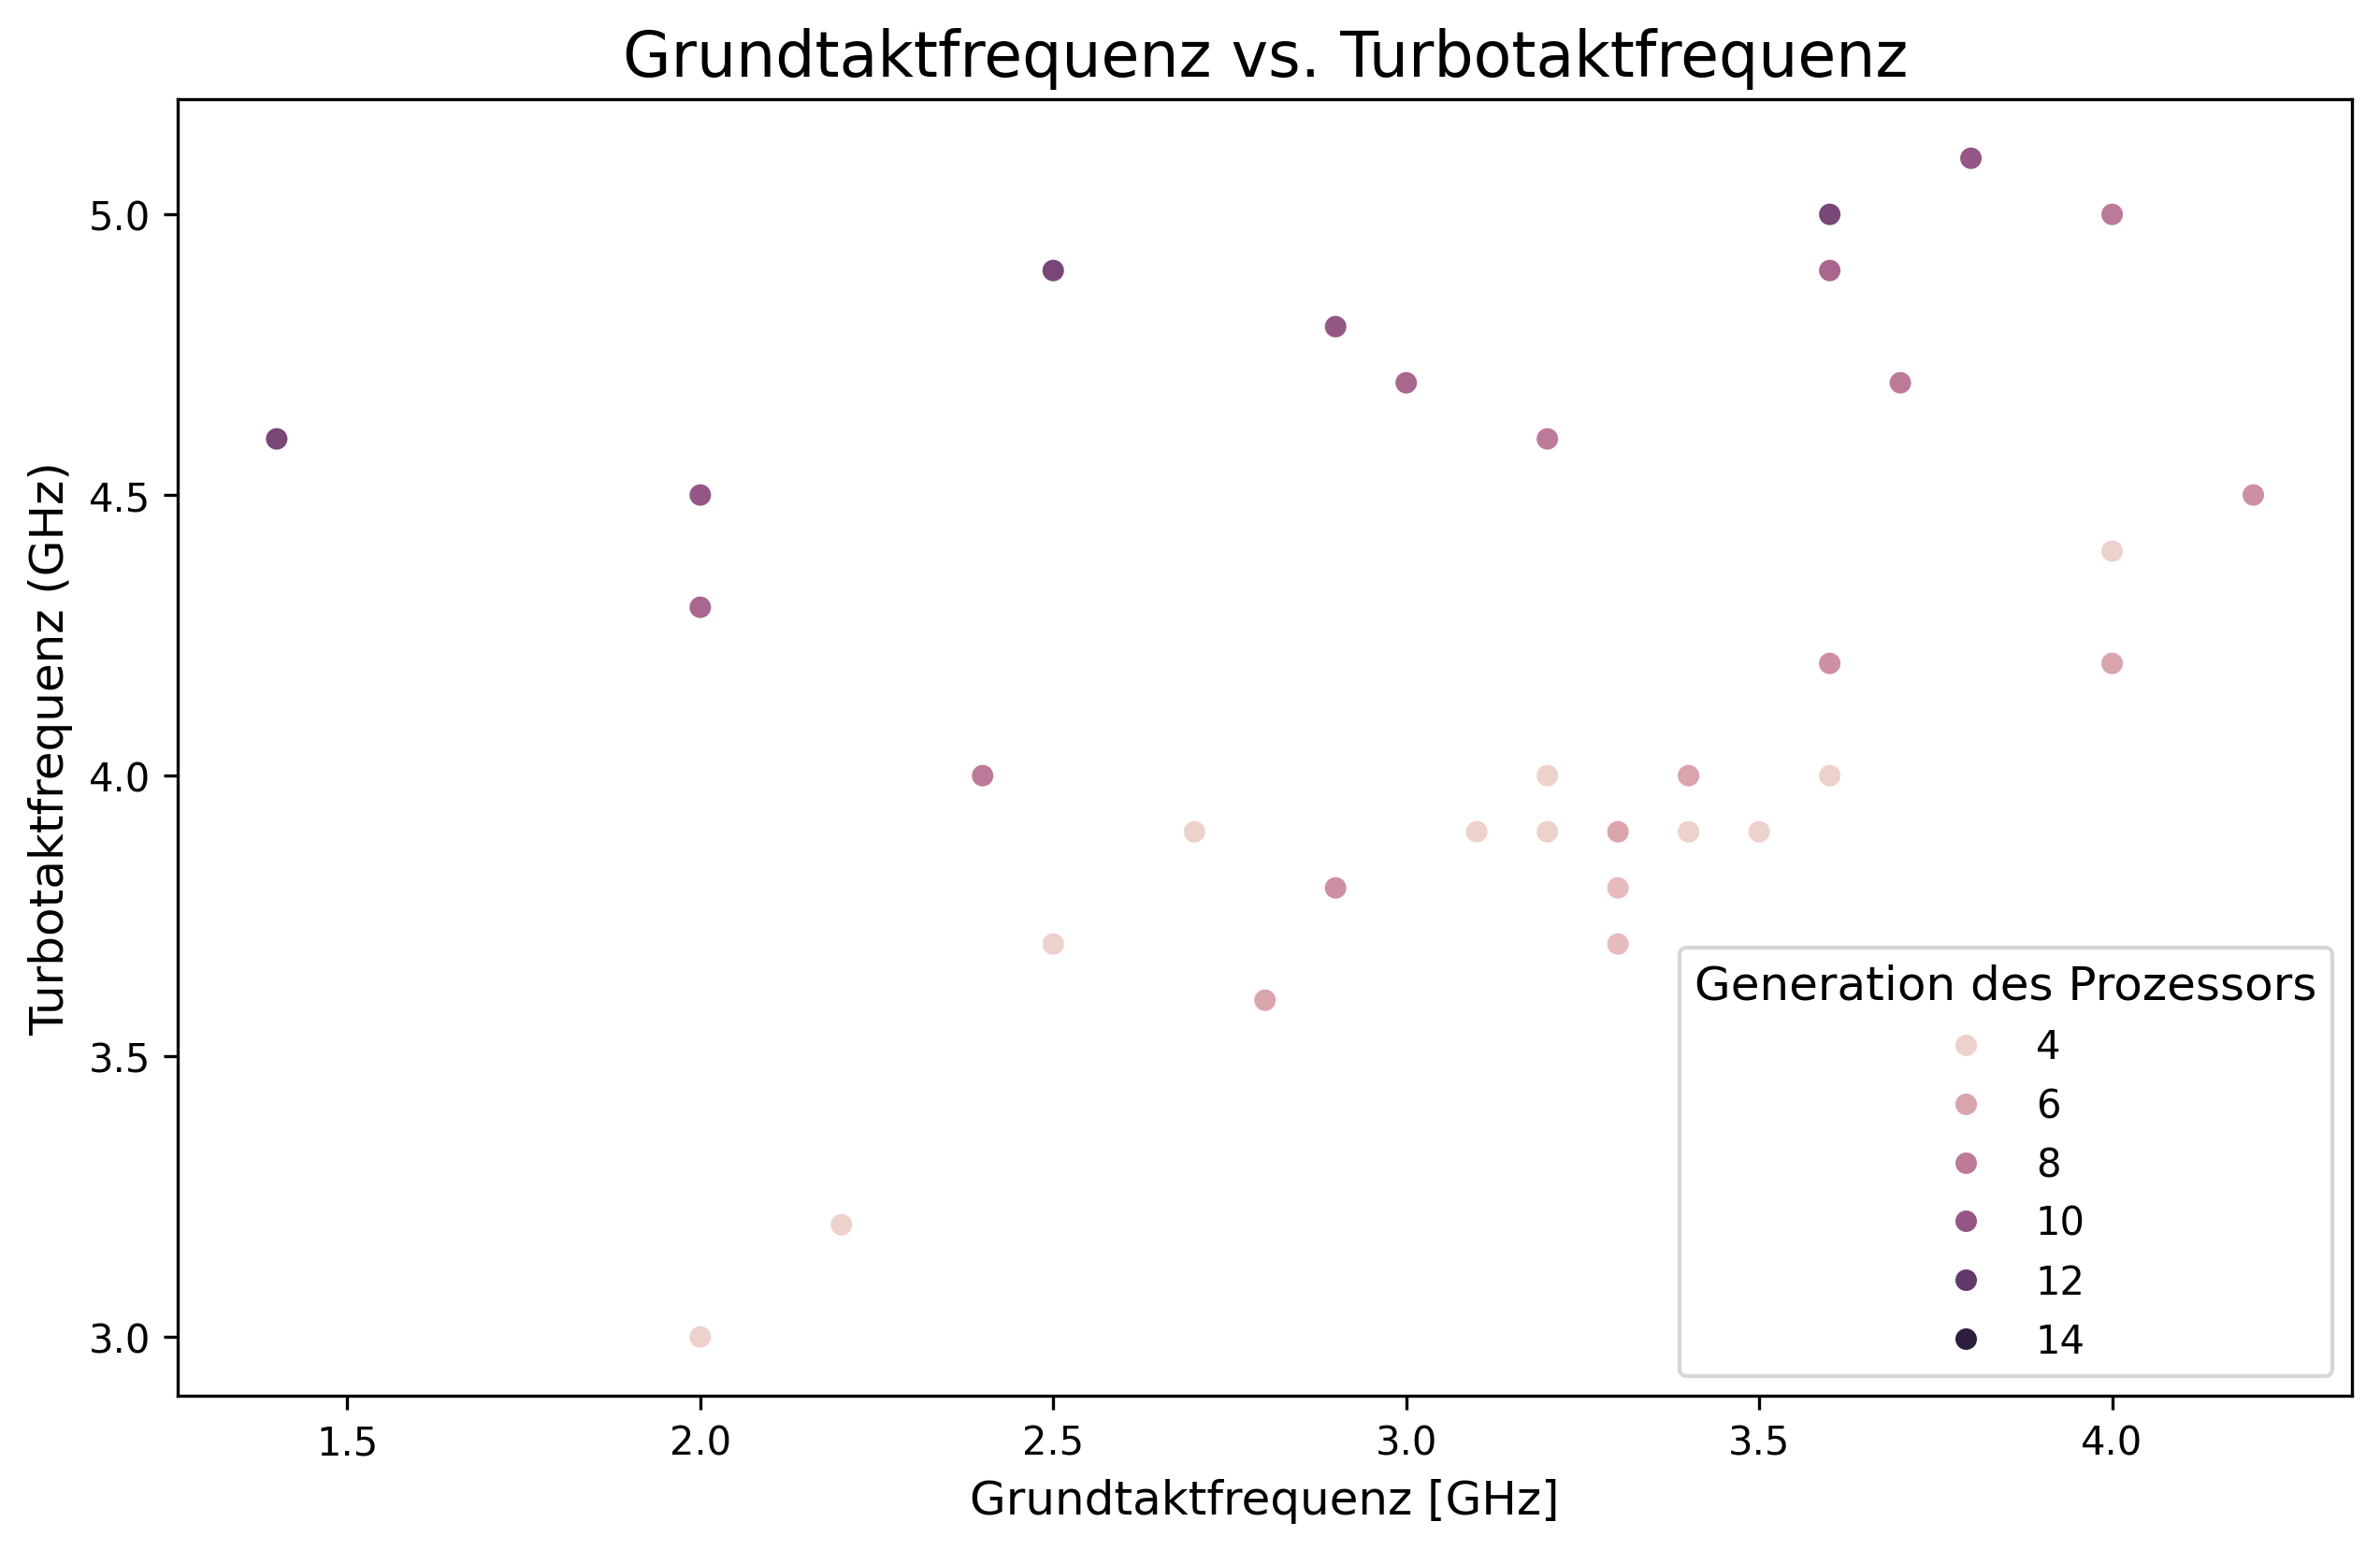
\includegraphics[width=\textwidth]{\imagedir/Scatterplot_Grundtaktfrequenz_vs_Turbotaktfrequenz.png} 
	\captionsetup{format=hang}
	\caption[Scatterplot]{\label{fig:scatterplot_Grundtaktfrequenz}Scatterplot erstellt mit \textit{matplotlib} und \textit{seaborn}}
\end{figure}

\begin{lstlisting}[caption={\texttt{Code für den Scatterplot in Figur 5.1}},captionpos=b]
    plt.figure(figsize=(10, 6))
    sn.scatterplot(data=df, x='grundtaktfrequenz_des_prozessors_GHz', y='max_turbo_taktfrequenz_GHz', hue='generation')
    plt.title("Grundtaktfrequenz vs. Turbotaktfrequenz", fontsize=16)
    plt.legend(title='Generation des Prozessors', fontsize=10, title_fontsize=12)
    plt.xlabel("Grundtaktfrequenz [GHz]", fontsize=12)
    plt.ylabel("Turbotaktfrequenz (GHz)", fontsize=12)
    plt.show()
\end{lstlisting}

Im Code wird zuerst ein neues Diagramm mit der Funktion \textit{plt.figure()} erstellt. Dabei wird die Größe des Diagramms auf 10x6 Zoll festgelegt. In Zeile
zwei wird mit der Funktion \textit{sn.scatterplot()} bereits der Scatterplot erstellt. Dabei wird als Datenquelle das im Kapitel \ref{sec:laden} erstellte DataFrame
\textit{df} verwendet. Die x-Achse wird mit der Spalte \textit{grundtaktfrequenz\_des\_prozessors\_GHz} und die y-Achse mit der Spalte \textit{max\_turbo\_taktfrequenz\_GHz}
belegt. Die Farbe des Punktes repräsentiert die Generation des Prozessors, welche in der im Kapitel \ref{sec:bereinigen} erstellten Spalte \textit{generation} gespeichert ist.
In den Spalten drei bis sechs werden der Titel, die Legende, sowie die Beschriftungen der x- und y-Achse festgelegt. Mit der Funktion \textit{plt.show()} in Spalte sieben wird
das Diagramm angezeigt.

Die restlichen Diagramme, die in dieser Arbeit erstellt wurden, sind nach einem ähnlichen Schema wie eben beschrieben erstellt worden. Dabei wurden unterschiedliche Diagrammtypen
sowie unterschiedliche Spalten des DataFrames verwendet. Alle Diagramme sind im Ordner \textit{Datenanalyse} in der Datei \textit{visualization.ipynb} zu finden.

% Fazit und Ausblick
% !TEX root =  master.tex
\chapter{Zusammenfassung}

\nocite{*}

Dieses Kapitel enthält die Zusammenfassung der Arbeit mit Fazit und Ausblick.

\section{Fazit}

...

\section{Ausblick}

...


%%%%%%%%%%%%%%%%%%%%%%%%%%%%%%%%%%%

%%%%%%%%%%%%%%%%%%%%%%%%%%%%%%%%%%%
% ANHÄNGE
%
% @stud: einzelne Anhänge bearbeiten und eigene Anhänge hier einfügen 
%        die nachfolgenden Zeilen deaktivieren, wenn keine Anhänge verwendet werden
%
\initializeAppendix

%%%%%%%%%%%%%%%%%%%%%%%%%%%%%%%%%%%

\singlespacing

%\ihead{}
%\printbibliography[title=\Literaturverzeichnis] 
\printbibliography 
\cleardoublepage

%\initializeBibliography
%%%%%%%%%%%%%%%%%%%%%%%%%%%%%%%%%%%

%%%%%%%%%%%%%%%%%%%%%%%%%%%%%%%%%%%
% INDEX
% @stud: ggf. Index auskommentieren, wenn nicht benötigt
%
\addcontentsline{toc}{chapter}{Index}
\printindex

\end{document}
